В результате пьезоэлектрического эффекта происходит деформация
кристаллической решетки. Данный эффект, очевидно, будет влиять на
КДО, а именно, на ее угловое положение и профиль.
Изменение профиля КДО может быть вызвано несколькими физическими процессами:

1. Изменение профиля может происходить за счет изменения структурного фактора при
пьезоэффекте. Данный эффект не рассматривается в рамках настоящей работы.
В первом приближении можно ограничиться случаем однородной деформации решетки
 кристалла. Такая деформация описывается
 матрицей пьезомодулей, вследствие чего относительное расположение атомов
 внутри элементарной ячейки остается постоянным, как и структурный фактор.

 \begin{figure}[H]
   \centering
   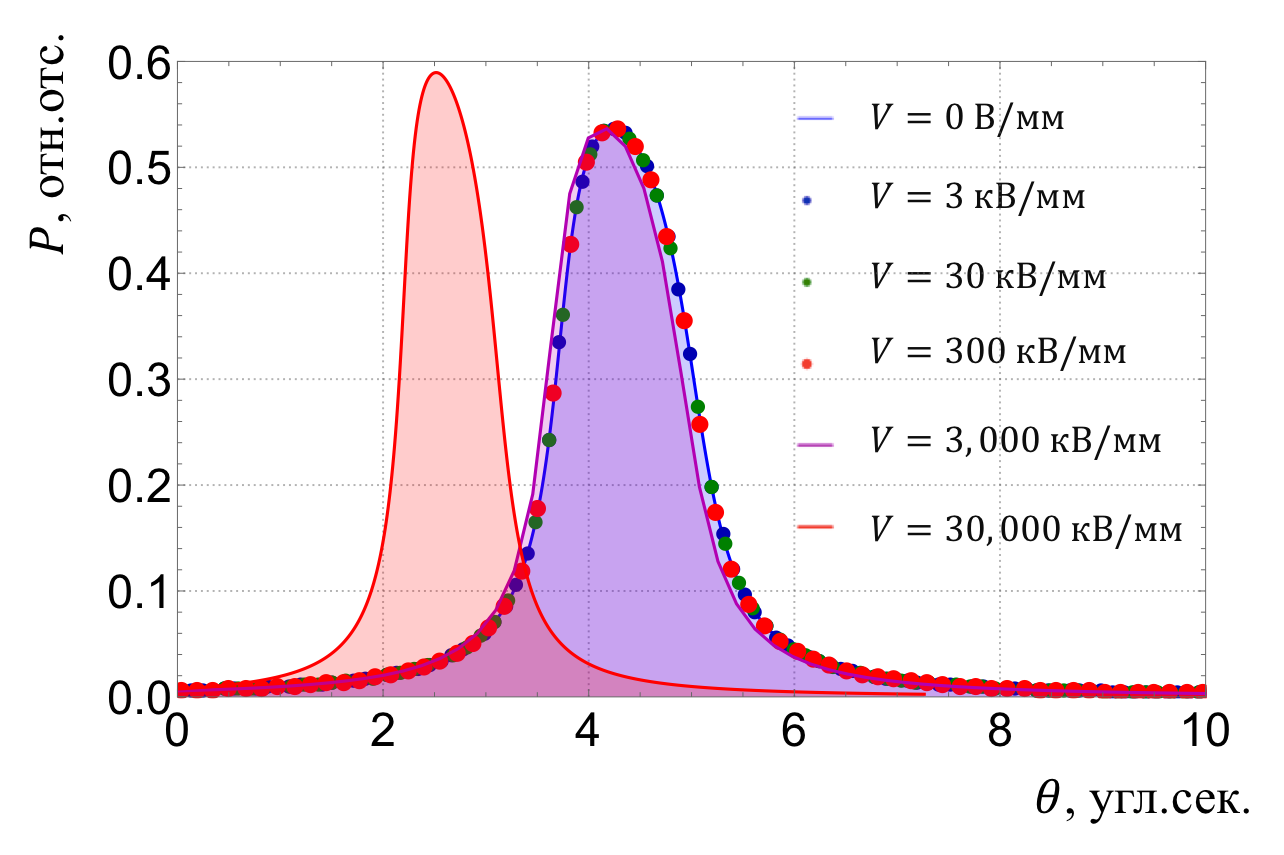
\includegraphics[width=0.6\textwidth]{images/self_kdo_under_ex_field.png}
   \caption{Изменение профиля собственной КДО для кристалла LGT(220)
   в зависимости от величины внешнего электрического поля для  $MoK_{\alpha}$ - излучения}
   \label{ris:self_kdo_deformation}
 \end{figure}

Стоит отметить, что учет анизатропии деформации решетки, вызванный различной чувствительностью
атомов разных сортов к электрическому полю, является актуальной и интересной задачей,
решение которой с помощью рентгеновской дифракции может стать существенным шагом
на пути понимания природы пьезоэффекта.

2. Профиль кривой также может изменяться вследствие изменения степени
 дисперсионности экспериментальной схемы.
При пьезоэффекте меняется межплоскостное расстояние образца, а значит и его угол Брэгга.
Таким образом, может возникать дисперсионное уширение или сужение КДО и изменение интегральной интесивности
отраженного пучка (см. \ref{sec:dispersion_cal_an_exp}) в зависимости
от увеличения или уменьшения разности углов Брэгга образца и монохроматора
под воздействием внешнего электрического поля. Для оценки этого эффекта был
проведен расчет, который заключался в оценке полуширины результирующей двухкристальной КДО
в зависимости от параметра решетки образца и, как следствие
 изменения угла Брэгга (рис. \ref{ris:FWHM_diference_bragg}).
%(отлажить по оси х дельта брэгга)
\begin{figure}[H]
  \centering
  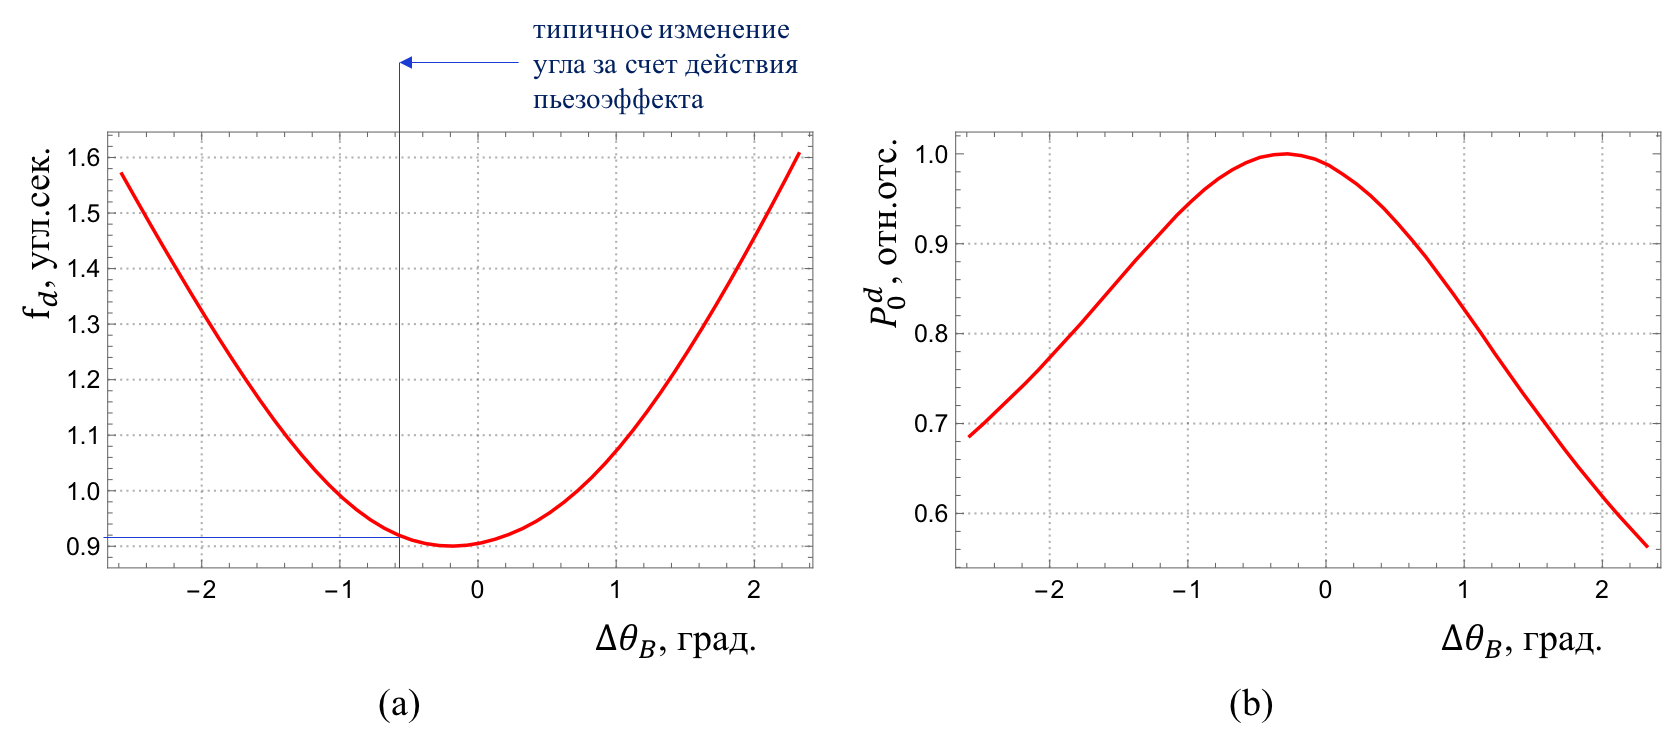
\includegraphics[width=0.95\textwidth]{images/delta_bragg_dispers.png}
  \caption{Зависимость полуширины двухкристальной КДО $f_d$ (a) и амплитуды в максимуме КДО  $P^d_0$ (b)
   от разности углов Брэгга $\Delta\theta_B =\theta_B^S-\theta_B^M $ кристаллов
  образца (S) и монохроматора (M). Углы Брэгга монохроматора Si (440) - $\theta_B^M = 21.6785 ^o$ и
   образца LGT(260) - $\theta_B^S = 21.0328 ^o$, источник $MoK_{\alpha}$ - излучение}
  \label{ris:FWHM_diference_bragg}
\end{figure}

На основании анализа полученных результатов можно сделать вывод, что минимальная полуширина
двухкристальной КДО соответсвует случаю, когда углы Брэгга обоих кристаллов в точности совпадают. С увеличением
дисперсионности схемы происходит монотонное увеличение полуширины КДО. Вместе с тем стоит отметить,
что при тех деформациях кристаллической решетки, которые возникают при пьезоэффекте,
изменение дисперсионности схемы настолько мало, что не приводит к видимому уширению КДО (рис. \ref{ris:FWHM_diference_bragg_KDO}).

\begin{figure}[H]
  \centering
  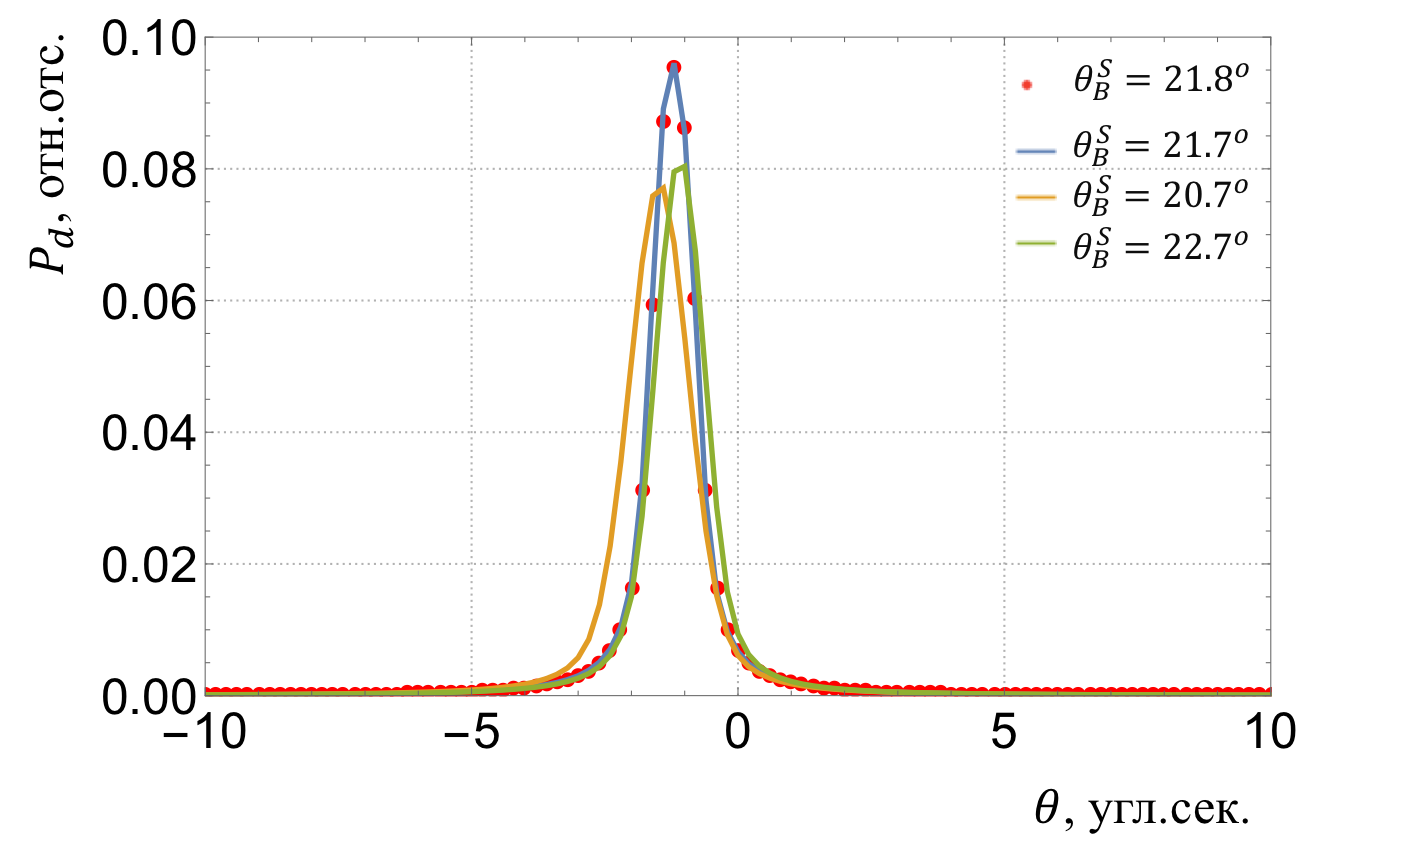
\includegraphics[width=0.8\textwidth]{images/FWHM_diference_bragg_KDO.png}
  \caption{КДО для разной степени дисперсионности схемы. Угол Брэгга кристалла - монохроматор
  Si(440) $\theta_B^M = 21.6785 ^o$, в качестве кристалла - образца LGT(260) $\theta_B^S = 21.0328 ^o$, $MoK_{\alpha}$ - излучение
  }
  \label{ris:FWHM_diference_bragg_KDO}
\end{figure}

Для того, чтобы добиться видимого изменения КДО, разница углов Брэгга образца и монохроматора
должна измениться на $1^o$, что соответсвует изменению межплоскостного расстояния на величину $d/d_0 \simeq 0.03$
процентов. Такие деформации параметра решетки не могут быть вызваны пьезоэффектом,
т.к. при относительном изменении параметра решетки $d/d_0 > 10^{-4}$ как правило
начинается разрушение кристаллической решетки. Таким образом в результате пьезоэффекта профиль кривой,
для рассмотренных нами случаев, можно считать постоянным.

Необходимо отметить, что изменение профиля КДО может происходить вследствие наличия
носителей зарядов (дефектов) в кристалле, которые под влиянием электрического поля
 могу деформировать кристаллическую решетку, но такой механизм
также не рассматривается в настоящей работе.

Данное заключение позволяется применять рассмотренные методы расчета для определения пьезоэлектрических констант,
а так же использовать времяразрешающий метод исследования (см. \ref{sec:slope_diff_piezo})
т.к. профиль кривой остается неизменным.
